In this section, we numerically study the performance of the centralized algorithms with different \me{\ell_q} values over multiple transmission slots. The system model examined for the illustrations is provided in Fig. \ref{fig-time-analysis}. For all users in the system, the average arrivals \me{A_k}'s are fixed and varied equally for the model considered in Fig. \subref*{fig-review}, and for Fig. \subref*{fig-review-time}, the average arrival is fixed to be \me{A_k = 6} bits. Note that the instantaneous arrivals \me{\lambda_k(i)} are all different and it follows the Poisson process. The \ac{PL} is modeled as a uniform random variable \me{[0,-6]} dB.
\begin{figure*}
	\centering
	\subfloat[][Average backlogged packets in the system after \me{250} transmission instants]{
		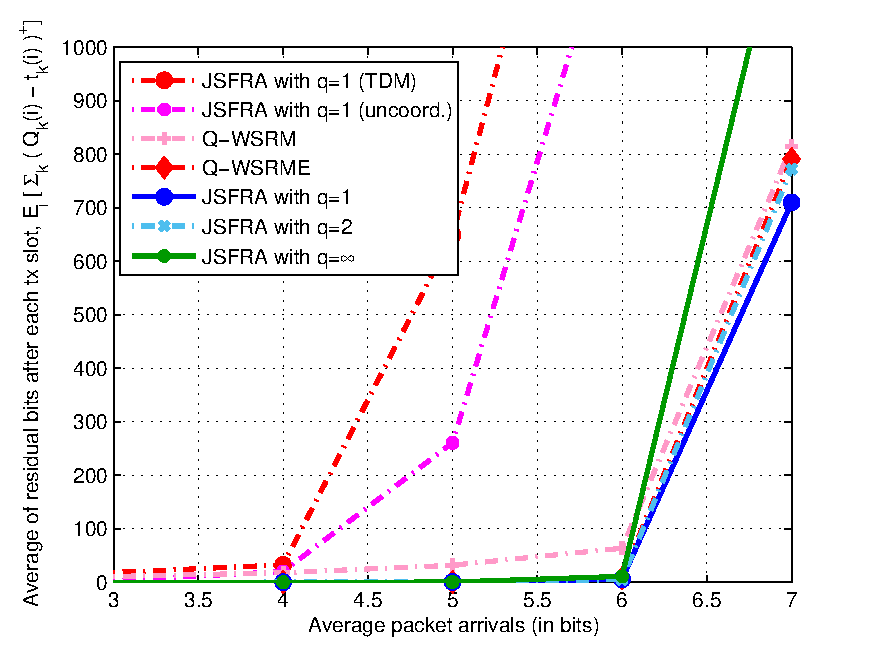
\includegraphics[width=0.48\textwidth]{average_queue_over_time-3}
		\label{fig-review}
	}
	\hfill
	\subfloat[][Total backlogged packets at each transmission slot for \me{A_k = 6} bits]{
		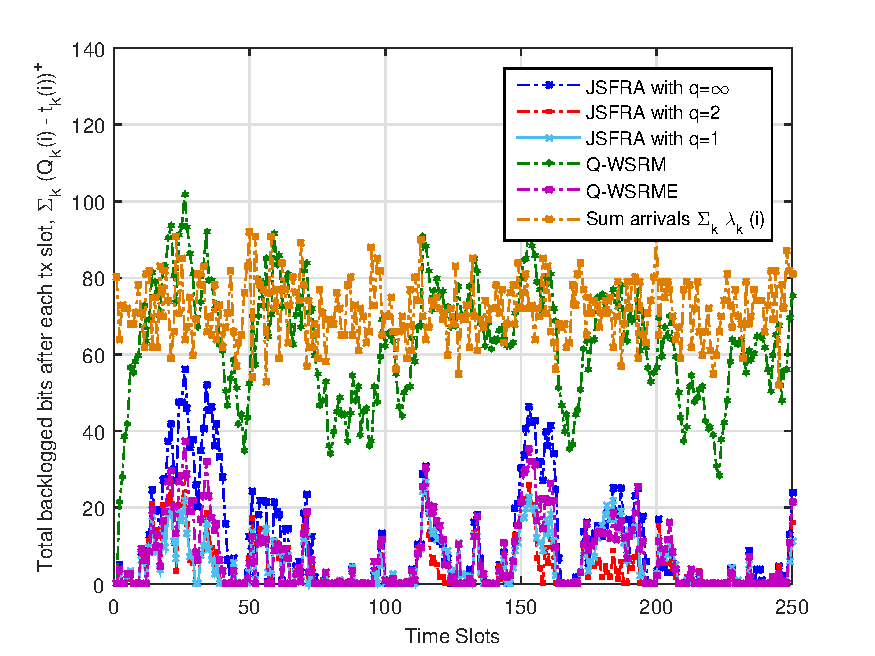
\includegraphics[width=0.48\textwidth]{instant_queue_over_time-4}
		\label{fig-review-time}
	}
	\caption{Time analysis of the Queue dynamics for a system \me{\lbrace N,N_B,K,N_T,N_R \rbrace = \lbrace 4,2,12,4,1 \rbrace}}
	\label{fig-time-analysis}
\end{figure*}

Fig. \subref*{fig-review} plots the average of the total number of backlogged packets left out in the system after each transmission instant, \textit{i.e}, \me{\mathbf{\mathbb{E}}_i \, [ \sum_k \left [ Q_k(i) - t_k(i) \right ]^+ ]}. Unlike the \ac{Q-WSRM} scheme, the average backlogged packets of the \me{\ell_2} \ac{JSFRA} scheme is comparable to the \ac{Q-WSRME} approach for all average arrival rates due to the explicit rate constraints \eqref{eqn-3.1.4}. However, when \me{A_k \geq 7} bits in Fig. \subref*{fig-review}, both \ac{Q-WSRM} and \ac{Q-WSRME} schemes perform the same since the problem of over-allocation is negligible. The performance of the \me{\ell_1} \ac{JSFRA} scheme outperforms all other schemes in terms of the average number of residual packets due to the greedy allocation at each instant. 

Fig. \subref*{fig-review} also includes the uncoordinated \me{\ell_1} \ac{JSFRA} scheme and the \ac{TDM} mode, which ignores the inter-cell interference terms in the \ac{SINR} expressions while designing the precoders. The performance of the \ac{TDM} scheme with the total power constraint is inferior to the uncoordinated transmission due to the diverse user \ac{PL} variations in the system model. Fig. \subref*{fig-review-time} compares the number of backlogged packets left in the system after each transmission slot by different centralized algorithms. The total number of residual packets for the \ac{Q-WSRM} scheme is noticeably large in comparison with the other schemes in Fig. \subref*{fig-review-time}. This performance loss is due to the inability in controlling the over-allocations at each instant. The instantaneous fairness constraint imposed by the \me{\ell_\infty} \ac{JSFRA} scheme is effective in reducing the number of backlogged packets for the average arrival rate considered in Fig. \subref*{fig-review-time}. However, in Fig. \subref*{fig-review}, the performance of the \me{\ell_\infty} \ac{JSFRA} is inferior to the \ac{Q-WSRM} scheme, since the fairness is not effective when the system is unstable, \textit{i.e}, when \me{A_k \geq 7} in the current model.
